\Author{\daAuthorTwo}

\subsubsection{OpenStreetMap}
The project OpenStreetMap (OSM) is an open-source initiative that aims to make high quality map data available to everyone for free. It was created in 2004 by Steve Coast. It was later widely adopted, with the main push being the pricing Google introduced to Google Maps, so that today it can be found in all kinds of application areas. Reaching from simple embedded web-components, all the way into video games like  the Microsoft Flight Simulator, which relies on OSM for it building models. The GIS behind OSM gets maintained by volunteers and is feed not only using GPS-Data but also image data and other different formats.\\ OSM is the backbone of this thesis and without it, it wouldn't have been possible to develop this tool.

\autocite{OSM:Wayback}
\autocite{OSM:wiki}


\begin{figure} [H]
    \center
    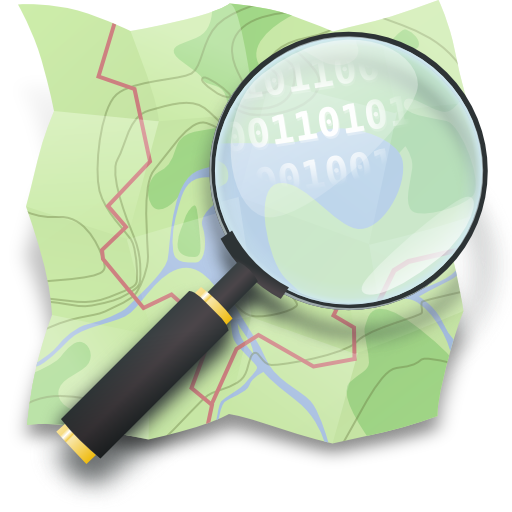
\includegraphics [width=0.4\textwidth] {images/Technologies/osmLogo.png}
    \caption{OSM Logo (Source: \url{https://wiki.openstreetmap.org/})}
\end{figure}

\subsubsection{GraphHopper}
GraphHopper (GH) in its core is an open-source routing engine written in Java. It can be deployed as a web server and is used to calculate the optimal route, distance or time between multiple different points. It supports multiple modes of transportation as well as "snap to road" technology. \autocite{GH:readMe} GH also provides a ready to go API that you can access for free, but we choose to deploy our own instance since the requests we needed to make exceed the limits of the free version.

\autocite{GH:installation}

\begin{figure} [H]
    \center
    
\includegraphics [width=0.4\textwidth] {images/Technologies/ghLogo.png}
    \caption{GraphHopper Logo (Source: \url{https://brandfetch.com/graphhopper.com})}
\end{figure}

\newpage